\clearpage
\section{Learning, Transitions, and Rule Sensitivity}
\label{app:diagnostics}

\begin{figure*}[t]
\centering
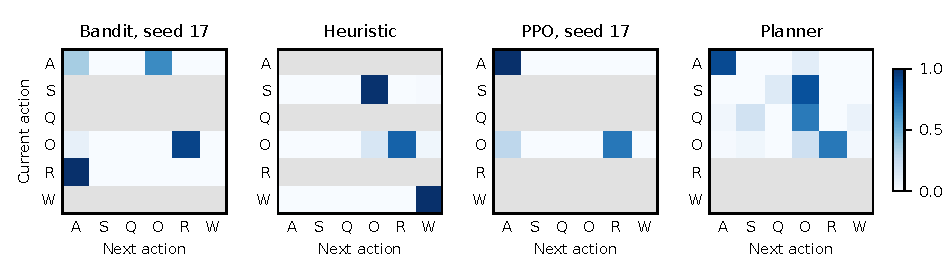
\includegraphics[width=\textwidth]{figures/assignment_transitions.pdf}
\caption{Within-episode action transitions in the initial test evaluation. A: ambiguity; S: signal; Q: question; O: any offer; R: ratify; W: withdraw. We merge six offer actions, then normalize each count row. Grey rows have no outgoing observations. All panels use the same scale.}
\label{fig:course_transitions}
\end{figure*}

\paragraph{Transition counts and interpretation.}
Figure~\ref{fig:course_transitions} summarizes saved action sequences, without connecting different episodes. Original eleven-action counts, weighted counts, and row probabilities are released in \texttt{transition\_matrices.json}; the figure's grouped counts accompany the paper. Counts describe enumerated response paths, not independent historical events or their population frequencies. The illustrative learned panels use seed 17.

Base PPO has 2,260 ambiguity-to-ambiguity transitions and 1,528 transitions from a 3:2 offer to ratification. The Bandit has 312 ambiguity repetitions and 672 transitions from 2:1 to ratification. The heuristic frequently moves from a signal to 2:2 (1,224 transitions); the planner often moves from a signal to 1:2 (836). These patterns connect the aggregate results to different strategic paths. In the implemented rules, ambiguity alone changes commitment status, not the counterpart's information response. Repeated ambiguity can therefore use opportunities without resolving uncertainty. The signal-to-offer pattern instead changes acceptance incentives before proposing terms. Frequencies summarize behavior; the matched cases in Appendix~\ref{app:discourse} provide the actual utterances and consequences.

\begin{figure*}[t]
\centering
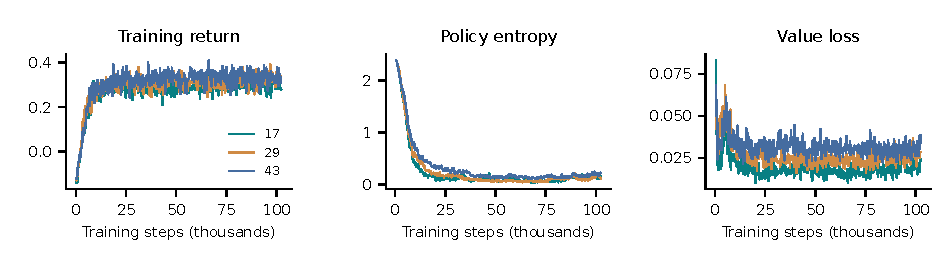
\includegraphics[width=\textwidth]{figures/assignment_learning.pdf}
\caption{Base PPO training diagnostics for seeds 17, 29, and 43. Return is the training logger's rolling episode mean. Entropy is the negative of the logged entropy loss; value loss is shown without additional smoothing. These are training diagnostics, not held-out performance.}
\label{fig:course_learning}
\end{figure*}

\paragraph{Learning stability.}
Training return rises from approximately $-0.14$ to $-0.12$ in the first logged episodes to 0.278, 0.339, and 0.308 at the final checkpoints (Figure~\ref{fig:course_learning}). Policy entropy falls from about 2.40 to 0.152, 0.125, and 0.228. Final value losses are 0.025, 0.028, and 0.039. The policy becomes more concentrated, but low entropy does not establish good negotiation: base PPO asks no questions and sends no signals on the initial test, and remains below the heuristic. Its test utility is $0.358\pm0.018$ across seeds. This motivates adding planner supervision rather than interpreting falling loss as sufficient evidence of success.

\begin{table}[t]
\centering\small
\begin{tabular}{lrrr}
\toprule
Changed rule & Planner & Questions & PPO \\
\midrule
$q=0.50$ & 0.527 & 0.00 & 0.410 \\
$q=0.70$ & 0.528 & 0.00 & 0.410 \\
$q=0.90$ & 0.532 & 1.00 & 0.410 \\
$q=1.00$ & 0.555 & 1.00 & 0.410 \\
$\delta=0.00$ & 0.486 & 1.00 & 0.410 \\
$\delta=0.10$ & 0.532 & 1.00 & 0.410 \\
$\delta=0.25$ & 0.596 & 1.00 & 0.410 \\
\bottomrule
\end{tabular}

\caption{One-factor evaluation-only rule shifts. Planner and PPO columns report utility; Questions is the planner's expected question count. PPO averages three frozen seeds. Other parameters are fixed to the reference configuration.}
\label{tab:course_sensitivity}
\end{table}

\paragraph{Information and rule sensitivity.}
Table~\ref{tab:course_sensitivity} separates question reliability from signal strength. The planner asks no question at reliability 0.5 or 0.7 and asks one at 0.9 or 1.0. Higher reliability becomes useful when it changes the preferred path enough to justify the question cost. Increasing the signal effect from 0 to 0.25 raises planner utility from 0.486 to 0.596. Base PPO stays at mean utility 0.410 across these shifts because it uses neither action in these evaluations. The frozen-policy design tests behavior under changed rules; it does not estimate what retraining would learn. Additional hard-type, rejection-cost, and question-cost sweeps are preserved in \texttt{sensitivity\_metrics.json}.

\begin{table*}[t]
\centering\small
\setlength{\tabcolsep}{3.5pt}
\begin{tabular}{lrrrrrrrrr}
\toprule
Policy & Own & Other & Cost & Break & Turns & Max $e$ & Mean $e$ & Reverse & Viol. \\
\midrule
Random & 0.147 & 0.040 & 0.292 & 0.890 & 4.288 & 0.856 & 0.547 & 0.437 & 0.000 \\
Bandit & 0.140 & 0.082 & 0.022 & 0.762 & 1.773 & 0.030 & 0.017 & 0.000 & 0.000 \\
Heuristic & 0.531 & 0.260 & 0.112 & 0.052 & 3.148 & 0.160 & 0.119 & 0.000 & 0.000 \\
PPO & 0.413 & 0.278 & 0.055 & 0.270 & 2.459 & 0.264 & 0.263 & 0.000 & 0.000 \\
Planner & 0.570 & 0.176 & 0.082 & 0.067 & 3.030 & 0.211 & 0.183 & 0.000 & 0.000 \\
\bottomrule
\end{tabular}

\caption{Additional initial-test metrics, averaged with the same event-group weighting as Table~\ref{tab:policies}A. Own and Other are pre-cost utilities averaged over all outcomes. Break is the breakdown rate, Reverse counts commitment reversals, and Viol. counts bilateral-acceptance violations. Escalation $e$ is a designed rejection index.}
\label{tab:course_metrics}
\end{table*}

\paragraph{Outcome quality and failure.}
Table~\ref{tab:course_metrics} reports both parties' utilities, costs, breakdowns, length, escalation, reversals, and violations. The planner's higher own net utility does not imply higher counterpart utility. No reported terminal agreement violates numerical acceptance conditions. The initial evaluation has a weighted infeasible fraction of 4.7\% under canonical offer and signal options, so withdrawal is not automatically a policy error. Initial discount, entropy, and reward-term training interventions are reported in Appendix~\ref{app:training}; their single-seed status is explicit.
